\begin{center}
    

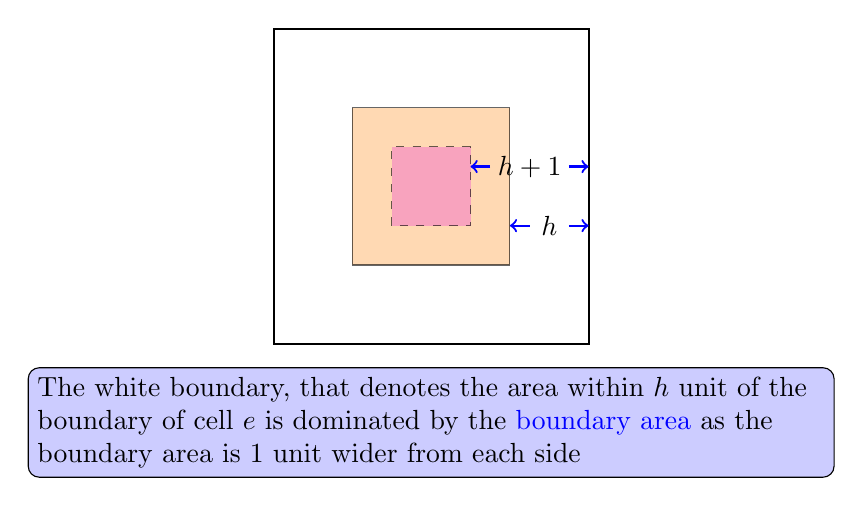
\begin{tikzpicture}

    % Square in the middle
    \draw[thick] (1, 1) rectangle ++(4, 4);
    \draw[fill=orange!50, opacity = 0.6] (2, 2) rectangle ++(2, 2);
    \draw[dashed, fill=magenta!50, opacity = 0.6] (2.5, 2.5) rectangle ++(1, 1);

    \draw[->, blue, thick ] (3.75,3.25) -- (3.5, 3.25) ;
    \draw[->, blue, thick ] (4.75,3.25)-- (5,3.25) ;
    \node at(4.25,3.25) {$h+1$};

    \draw[->, blue, thick ] (4.25,2.5)-- (4,2.5) ;
    \draw[->, blue, thick ] (4.75,2.5)-- (5,2.5) ;
    \node at(4.5,2.5) {$h$};
    
    \node[draw, fill=blue!20, text width=10cm, rounded corners] at (3, 0) {
    The white boundary, that denotes the area within \textbf{$h$} unit of the boundary of cell $e$ is dominated by the \textcolor{blue}{boundary area} as the boundary area is 1 unit wider from each side};

\end{tikzpicture}

\end{center}